\documentclass[a4paper]{article}
\usepackage[warn]{mathtext}
\usepackage[utf8]{inputenc}
\usepackage[T2A]{fontenc}

\usepackage[english,russian]{babel}
\usepackage{multicol}
\usepackage{fancyhdr}
\usepackage{graphicx}
\usepackage{microtype}
\usepackage{wrapfig}
\usepackage{amsmath}
\usepackage{floatflt}
\usepackage{geometry} \geometry{verbose,a4paper,tmargin=2cm,bmargin=2cm,lmargin=1.5cm,rmargin=1.5cm}
\usepackage{float}
\usepackage{amssymb}
\usepackage{caption}
\usepackage{epsfig}
\usepackage{newunicodechar}

\begin{document}

\graphicspath{ {pictures/} }

\begin{titlepage}
	\centering
	\vspace{5cm}
    {\scshape\LARGE Московский физико-технический институт\par}
	\vspace{5cm}
	{\scshape\Large Лабораторная работа по общей физике \par}
	\vspace{1cm}
    {\huge\bfseries  8.1 Определение постоянных Стефана-Больцмана и Планка из анализа
    теплового излучения накаленного тела \par}
	\vspace{1cm}
	\vfill
    \begin{flushright}
        {\large выполнил студент Б04-852 группы ФЭФМ}\par
        \vspace{0.3cm}
        {\LARGE Яромир Водзяновский}
    \end{flushright}
	\vfill
Долгопрудный, 2020
% Bottom of the page
\end{titlepage}

\pagestyle{fancy} 
\fancyhead[R]{Тепловое излучение накаленного тела }
\fancyhead[L]{Квантовая физика   $\sim  \hat(\, ^{\circ} 0  ^{\circ} \, \hat) \sim$}
\fancyhead[C]{}
\fancyfoot[C]{ \noindent\rule{\textwidth}{0.4pt} \thepage }

\tableofcontents

\newpage



\section{Цель работы}

\begin{itemize}
    \item При помощи модели абсолютного черного тела провести измерения температуры оптическим пирометром
    с исчезающей нитью и термопарой
    \item Исследовать ищлучение накаленных тел с ращзличной испускательной способностью
    \item Определить постоянные Планка и Стефана-Больцмана
\end{itemize}



\section{Оборудование}

\begin{itemize}
    \item Оптический пирометр
    \item Вольфрамовая лампа
    \item Неоновая лампа
    \item Образцы колец
    \item Модель АЧТ
    \item Блок питания
    \item Вольтметры
    \item Библиотеки numpy, scipy, matplotlib, pandas в python 3 для обработки данных
\end{itemize}



\section{Теория}

Для измерения температуры разогретых тел, можно применять методы оптической пирометрии, основанные 
на зависимости испускательной спосоьности от температуры. Различают три температуры, функционально 
связанные с истинной термодинамической температурой и излучательной способнотью тела:

\begin{enumerate}
    \item \textbf{Радиационную} $T_{\text{рад}}$ - температура АЧТ, при которой его интегральная 
    испускательная способнасть = интегральной испускательной способности исследуемого тела.
    \item \textbf{Цветовую} $T_{\text{цв}}$ - температура АЧТ, при которой отношение их спектральных 
    испускательных способностей для двух заданных длин волн одинаково.
    \item \textbf{Яркостную} $T_{\text{ярк}}$ - температура АЧТ, при которой его спектральная испускательная
    способность равна спектральной испускательной способности исследуемого тела при той же длине волны.
    Именно эту температуру мы будем измерять. 
\end{enumerate}

Измерение яркостной температуры производиться с помощью оптического пирометра с исчезающей нитью,
мы визуально сравниваем яркость нити с яркостью исследуемого тела. Равенство  видимых яркостей наблюдается 
через монохроматический светофильтр ($\lambda = 6500 \stackrel{\circ}{A}$) фиксируется по исчезновению
нити на фоне расскаленного тела. \par

Температура нти решулируется силой тока через нее. Шкалу прибора, измеряющего ток через нить градуируют
по АЧТ, теормодинамическую температуру которого измеряют через термопару. Если тело, температуру которого
мы хотим измерить излучает как АЧТ, то мы можем с помощью пирометр найти его температуру. Если тело излучает по другому,
то мы найдем его яркостную температуру. Яркостная температура вскегда ниже чем термодинамическая, т.к. 
любое нечерное тело излучает меньше, чем АЧТ при той же температуре. \par 

В этой работе используем прирометр проградуированный при изготовлении по АЧТ. Вначале с помощью модели АЧТ 
проверим правильность работы пирометра, а затем с его помощью исследуем излучение различных материалов. Необходимая для оьработки 
данных зависимость между яркостной и термодинамической температурами для вольфрама на рис. \ref{p1}

\begin{figure}[H]
    \begin{center}
    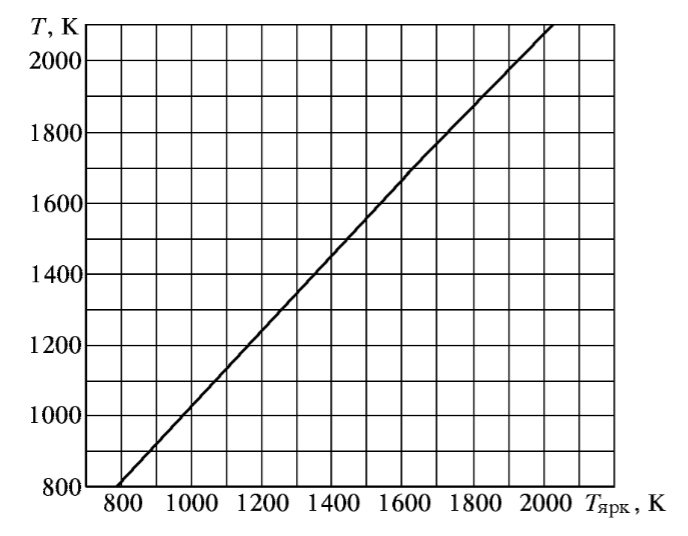
\includegraphics[scale = 0.8]{p1.png}
    \caption{График зависимости $T = f(T_{\text{ярк}})$ для вольфрама}
    \label{p1}
    \end{center}
\end{figure}

По результатам измреения сможем судить о справедливости закона Стефана-Больцмана. Приравняем мощность, 
потребляемую нитью к излучаемому ею за еденицу времени кол-ву энергии. Если бы нить была АЧТ:

\begin{equation}
    W = \sigma S (T^4 - T_0^4),
\end{equation}

где $W$ - потребляемая мощность, $S$ - площадь, $T$ - температура нити,  $T_0$ - температура окр. среды.\par

Однако вольфрам является серым телом, т.е. спектр излучения подобен спектру АЧТ, но ослаблен в $\varepsilon_T$ раз:

\begin{equation}
    W = \varepsilon_T S \sigma T^4
\end{equation}

Значение коэффициента излучениея $\varepsilon_T$ от температуры приведена на рис. \ref{p2}

\begin{figure}[h]
	\begin{center}
	\begin{minipage}[h]{0.4\linewidth}
	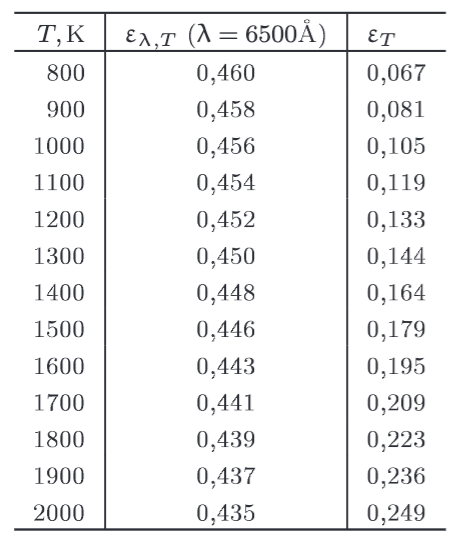
\includegraphics[width=1\linewidth]{p2.png}
	\caption{Поправочный коэффициенты излучения для вольфрама} 
	\label{p2}
	\end{minipage}
	\hfill 
	\begin{minipage}[h]{0.45\linewidth}
	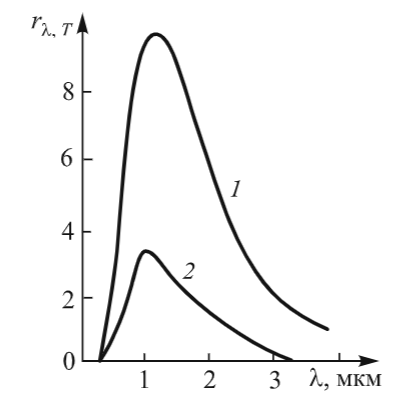
\includegraphics[width=1\linewidth]{p3.png}
	\caption{Распределение энергии в спеткре излучения: 1 - АЧТ, 2 - вольфрам. T = 2450 К}
	\label{p3}
	\end{minipage}
	\end{center}
\end{figure}

Измерив температуру вольфрамовой нити от подводимой мощности можно проверить закон С-Б, т.е. построить $W(T)$ в логарифмическом
мастштабе и получиь тпоказатель степени $n \approx 4$ как коэф. наклона. А из ф-лы (2) можно найти $\sigma$. \par

Однако оличие полученных эксперементально величин может не совпадать с теорией по причине селективности излучения 
вольфрама: при T = 2400 K, излучение видимой облатси спеткра существенно больше, чем следует из распеределения Планка. Эта 
разница отображена на рис. \ref{p3}. \par 

Проведя измерения в диапазоне 800 - 1500 $^{\circ C}$ получим значения $\sigma$ и $n$ достаточно точно.



\section{Экспериментальная установка}

Экпериментальная установка (рис. \ref{setup})

\begin{figure}[H]
    \begin{center}
    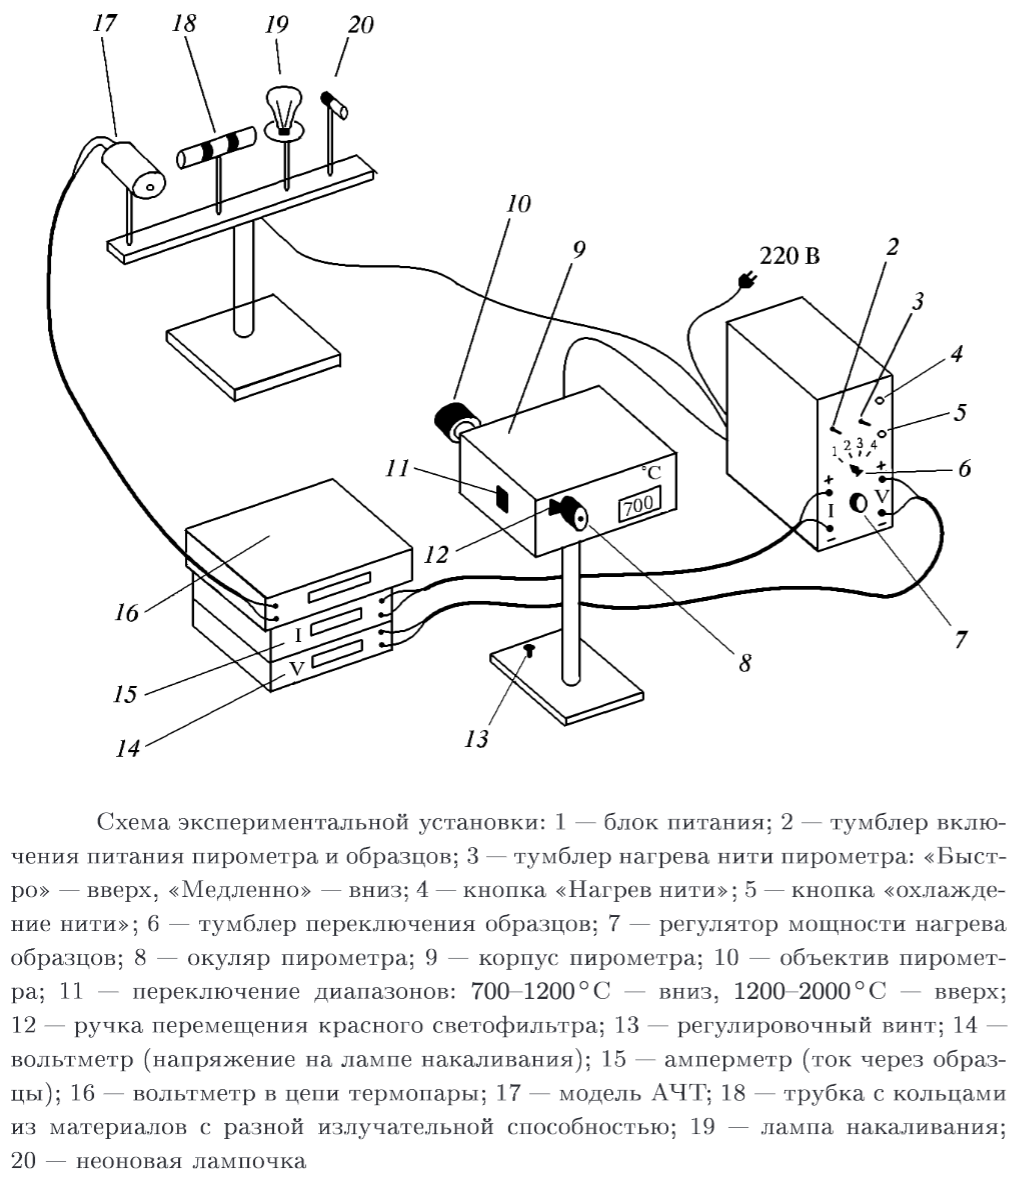
\includegraphics[scale = 0.6]{setup.png}
    \caption{}
    \label{setup}
    \end{center}
\end{figure}

Модель АЧТ представляет собой керамическую трубку диаметром 3 мм и длиной 50 мм, закрытую с одного конца и окруженную внешним кожухом.
Нагрев трубки осуществляется намотанной на нее нихромовой спиралью, питаемой от источника тока. 
Температура АЧТ измеряется хромельалюмелевой термопарой, один спай находится в дне трвьки, а другой 
в вольтметре, измерящего ЭДС термопары.\par 

В работе используется три образца. Один образец в виде керамической трубки с набором колец 
из различных материалов, спираль может нагреваться до 1000 $^{\circ} C$. \par 

Другой образец - вольфрамовая нить электрической лампочки. Сила тока через нить измеряется амперметром 15, падение 
напяржения на ссамой нити измяется вольтметром 16. Так мы сможем определить мощность подаваему на нить. 



\section{Ход работы}



\subsection{Изучение работы оптического пирометра}



В этой части работы с помощью пирометра измеряется темература модели АЧТ и проводится сравнение
ее значения со значением температуры термопарного термометра. 

\begin{enumerate}
    \item Выведем серый и красный светофильтры из пирометра.
    
    \item Подключим пирометр к сети и доведем показания до $\sim 900 - 950 ^{\circ} C$. В окуляре
    увидим раскаленную нить. \par
    Направим пирометр на модель АЧТ, подадим на него напряжение и максимальную мощность, через 10-15 мин. 
    оно нагреетс и мы должны увидеть четкое изображение дна модели. 

    \item Введем красный фильтр пирометра.

    \item Определим по шкале пирометра значения яркостной температуры АЧТ.  Одновременно опредлим 
    температуру АЧТ по термопаре  и цифрового вольтметра 16. Постоянная термопары 41 мкВ/$^{\circ} C$.

    $$t_{\text{пир}} \approx 920 ^{\circ} C$$

    $$t_{\text{тп}} = \frac{39.51\; B}{41 \; \text{мкВ/}^{\circ} C} \approx 964 \; ^{\circ} C$$

    Показания отличаются менее чем на 5\%
\end{enumerate}



\subsection{Измерение яркостной температуры накаленных тел}



Этот эксперимент покажет, что различные тела, накаленные до одинаковой термодинамической температуры,
имеют различную яркостную температуру.\par 

\begin{enumerate}
    \item Направим пирометр на поверхность керамической трубки с кольцами из различных материалов;
    также как и в предыдущем опыте поставим мощность прогрева на максимум и прогреем трубку до каления.

    \item Измерим яркостную температуру поверхности трубки и каждого из колец. На рис. \ref{rings} изображены кольца и трубка,
    где виден котраст яркости колец.
    \begin{figure}[H]
        \begin{center}
        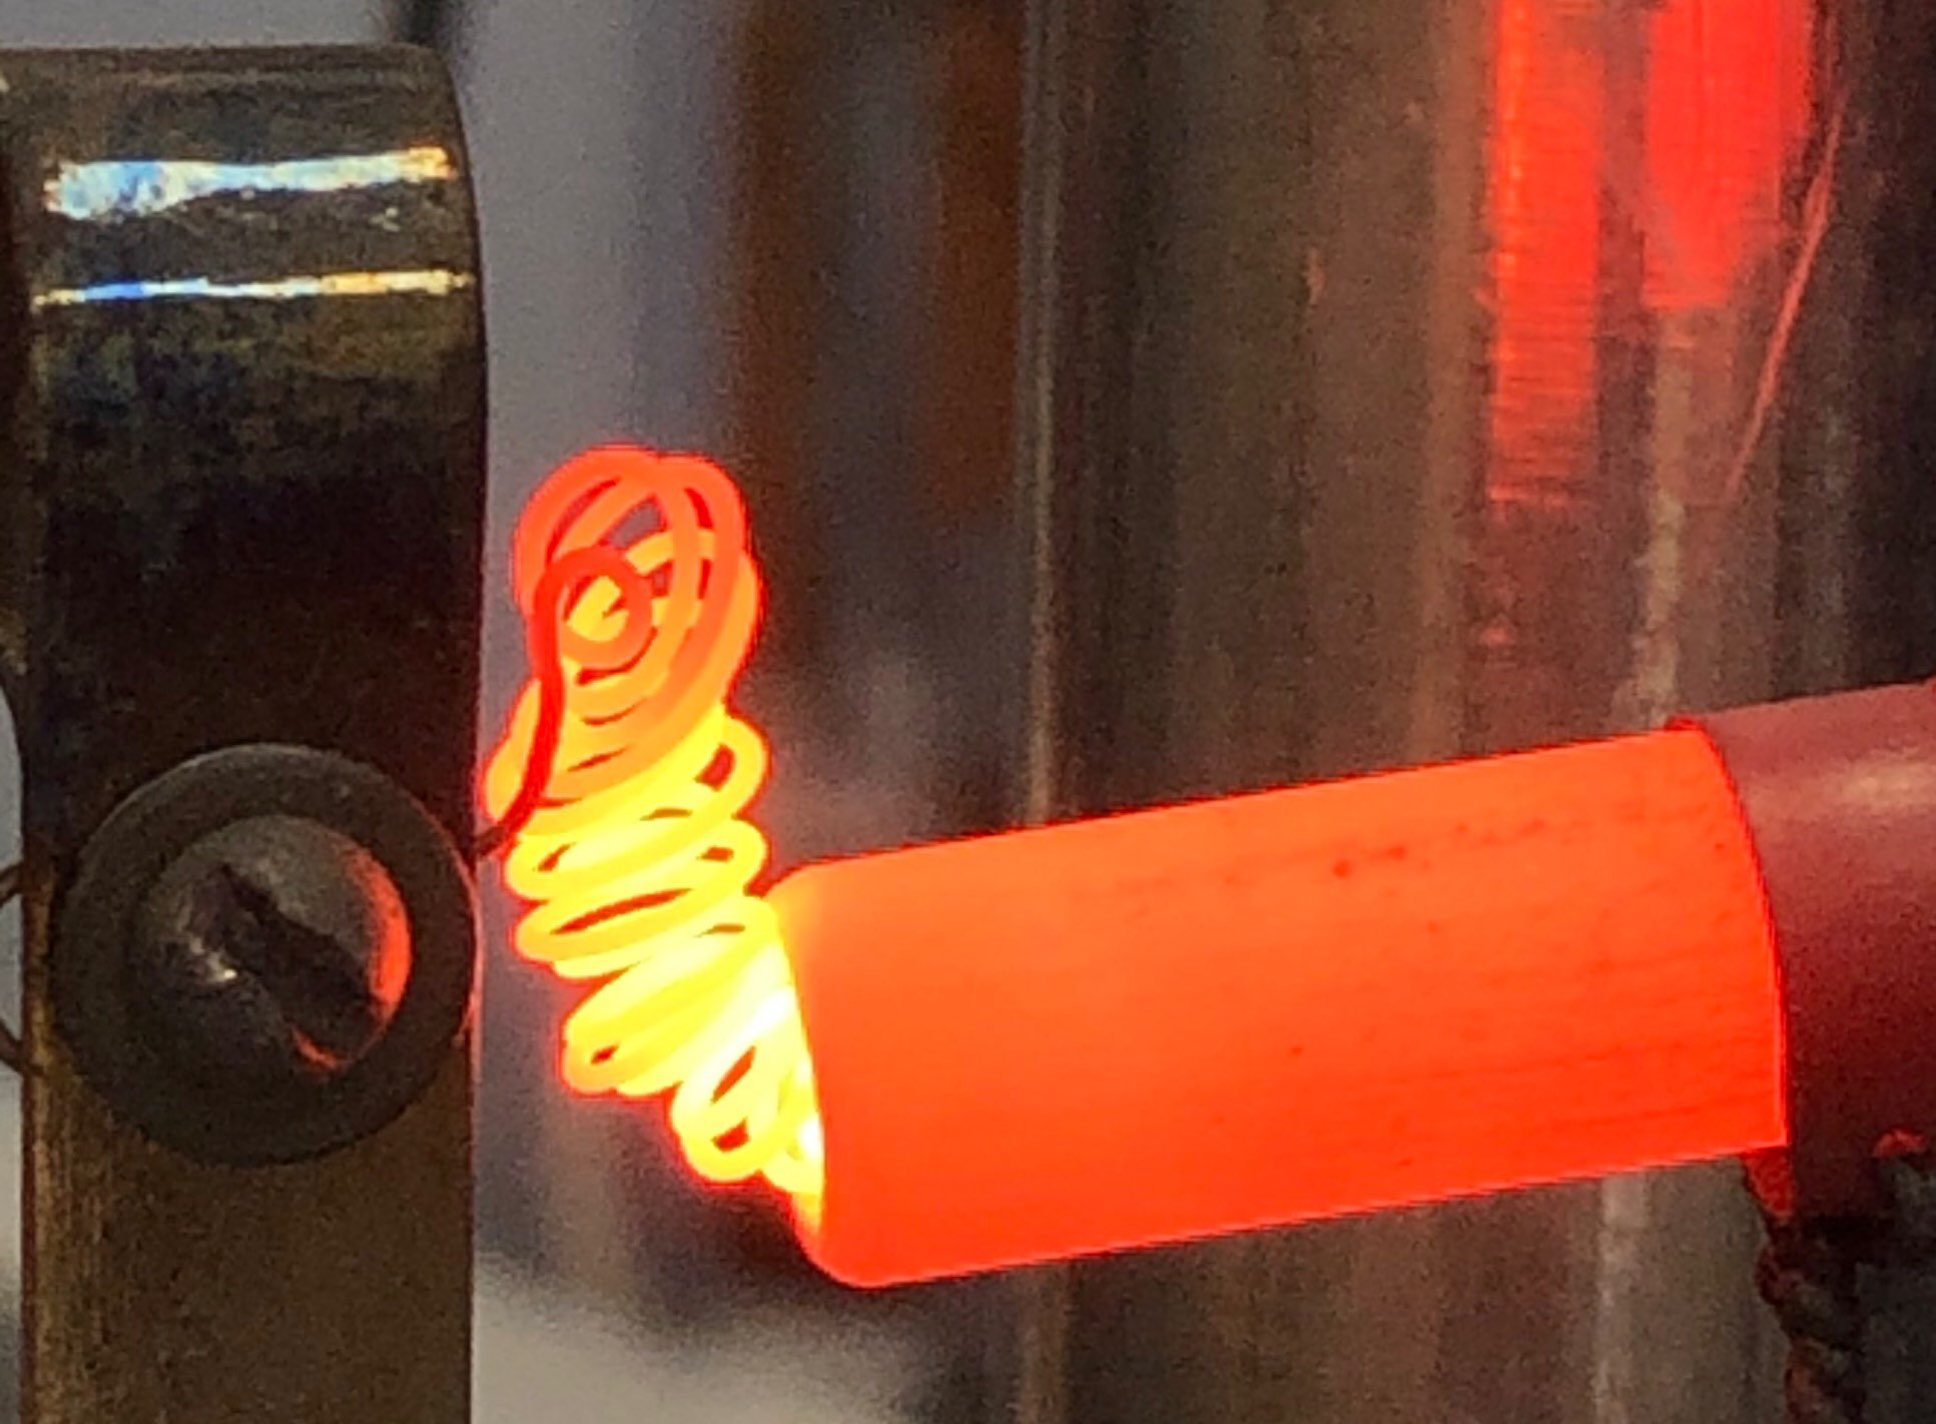
\includegraphics[scale = 0.1]{rings.jpg}
        \caption{Фото колец и трубки}
        \label{rings}
        \end{center}
    \end{figure}
    $$t_{тр} \approx 915 ^{\circ} C$$

\end{enumerate}



\subsection{Проверка закона Стефана-Больцмана}



\begin{enumerate}
    \item Направим прирометр на нить лампы накаливания.
    
    \item Постепенно увеличивая накал нити лампы, начиная со слабого накала $\sim  900 ^{\circ} C$ вплоть до $1900 ^{\circ} C$. 
    Будем измерять яркостную температуру через каждые 100 $^{\circ} C$, а также записывать падение напряжения и величину тока. 
    Занесем данные в таблицу \ref{t1}. 
    \begin{table}[h]
        \centering
        \caption{}
        \label{t1}
        \begin{tabular}{|c|c|c|c|c|c|}
            \hline
           $T_{\text{ярк}}$, K & $T_{\text{терм}}$, K & $I$, mA & $U$, B & $W$, мВт \\\hline \hline
            1173 & 1242 & 0.70 & 22.86 & 16.00 \\ \hline
            1273 & 1348 & 0.76 & 27.85 & 21.25 \\\hline
            1373 & 1454 & 0.80 & 30.94 & 24.75 \\\hline
            1423 & 1507 & 0.83 & 33.80 & 27.92 \\\hline
            1473 & 1560 & 0.87 & 36.85 & 32.06 \\\hline
            1573 & 1666 & 1.02 & 50.07 & 51.07 \\\hline
            1673 & 1771 & 1.07 & 55.70 & 59.71 \\\hline
            1723 & 1824 & 1.13 & 61.35 & 69.33 \\\hline
            1773 & 1877 & 1.19 & 67.10 & 79.65 \\\hline
            1823 & 1930 & 1.27 & 76.00 & 96.52 \\\hline
            1873 & 1983 & 1.31 & 81.40 & 106.63 \\\hline
            1973 & 2089 & 1.41 & 92.70 & 130.71 \\\hline
            2023 & 2142 & 1.47 & 99.50 & 146.27 \\\hline
            2073 & 2195 & 1.53 & 106.90 & 163.56 \\\hline
            2123 & 2248 & 1.61 & 117.60 & 189.34 \\\hline
            2173 & 2301 & 1.67 & 125.00 & 208.75 \\\hline
        \end{tabular}
    \end{table}

    \item Для каждого значения яркостной температуры по графику на рис. \ref{p1} определим термодинамиескую 
    тепературу (занесем резузльтат в таблицу \ref{t1}) и построим график $W = f(T_{\text{терм}})$ на рис. \ref{graph1}
    \begin{figure}[h]
        \begin{center}
        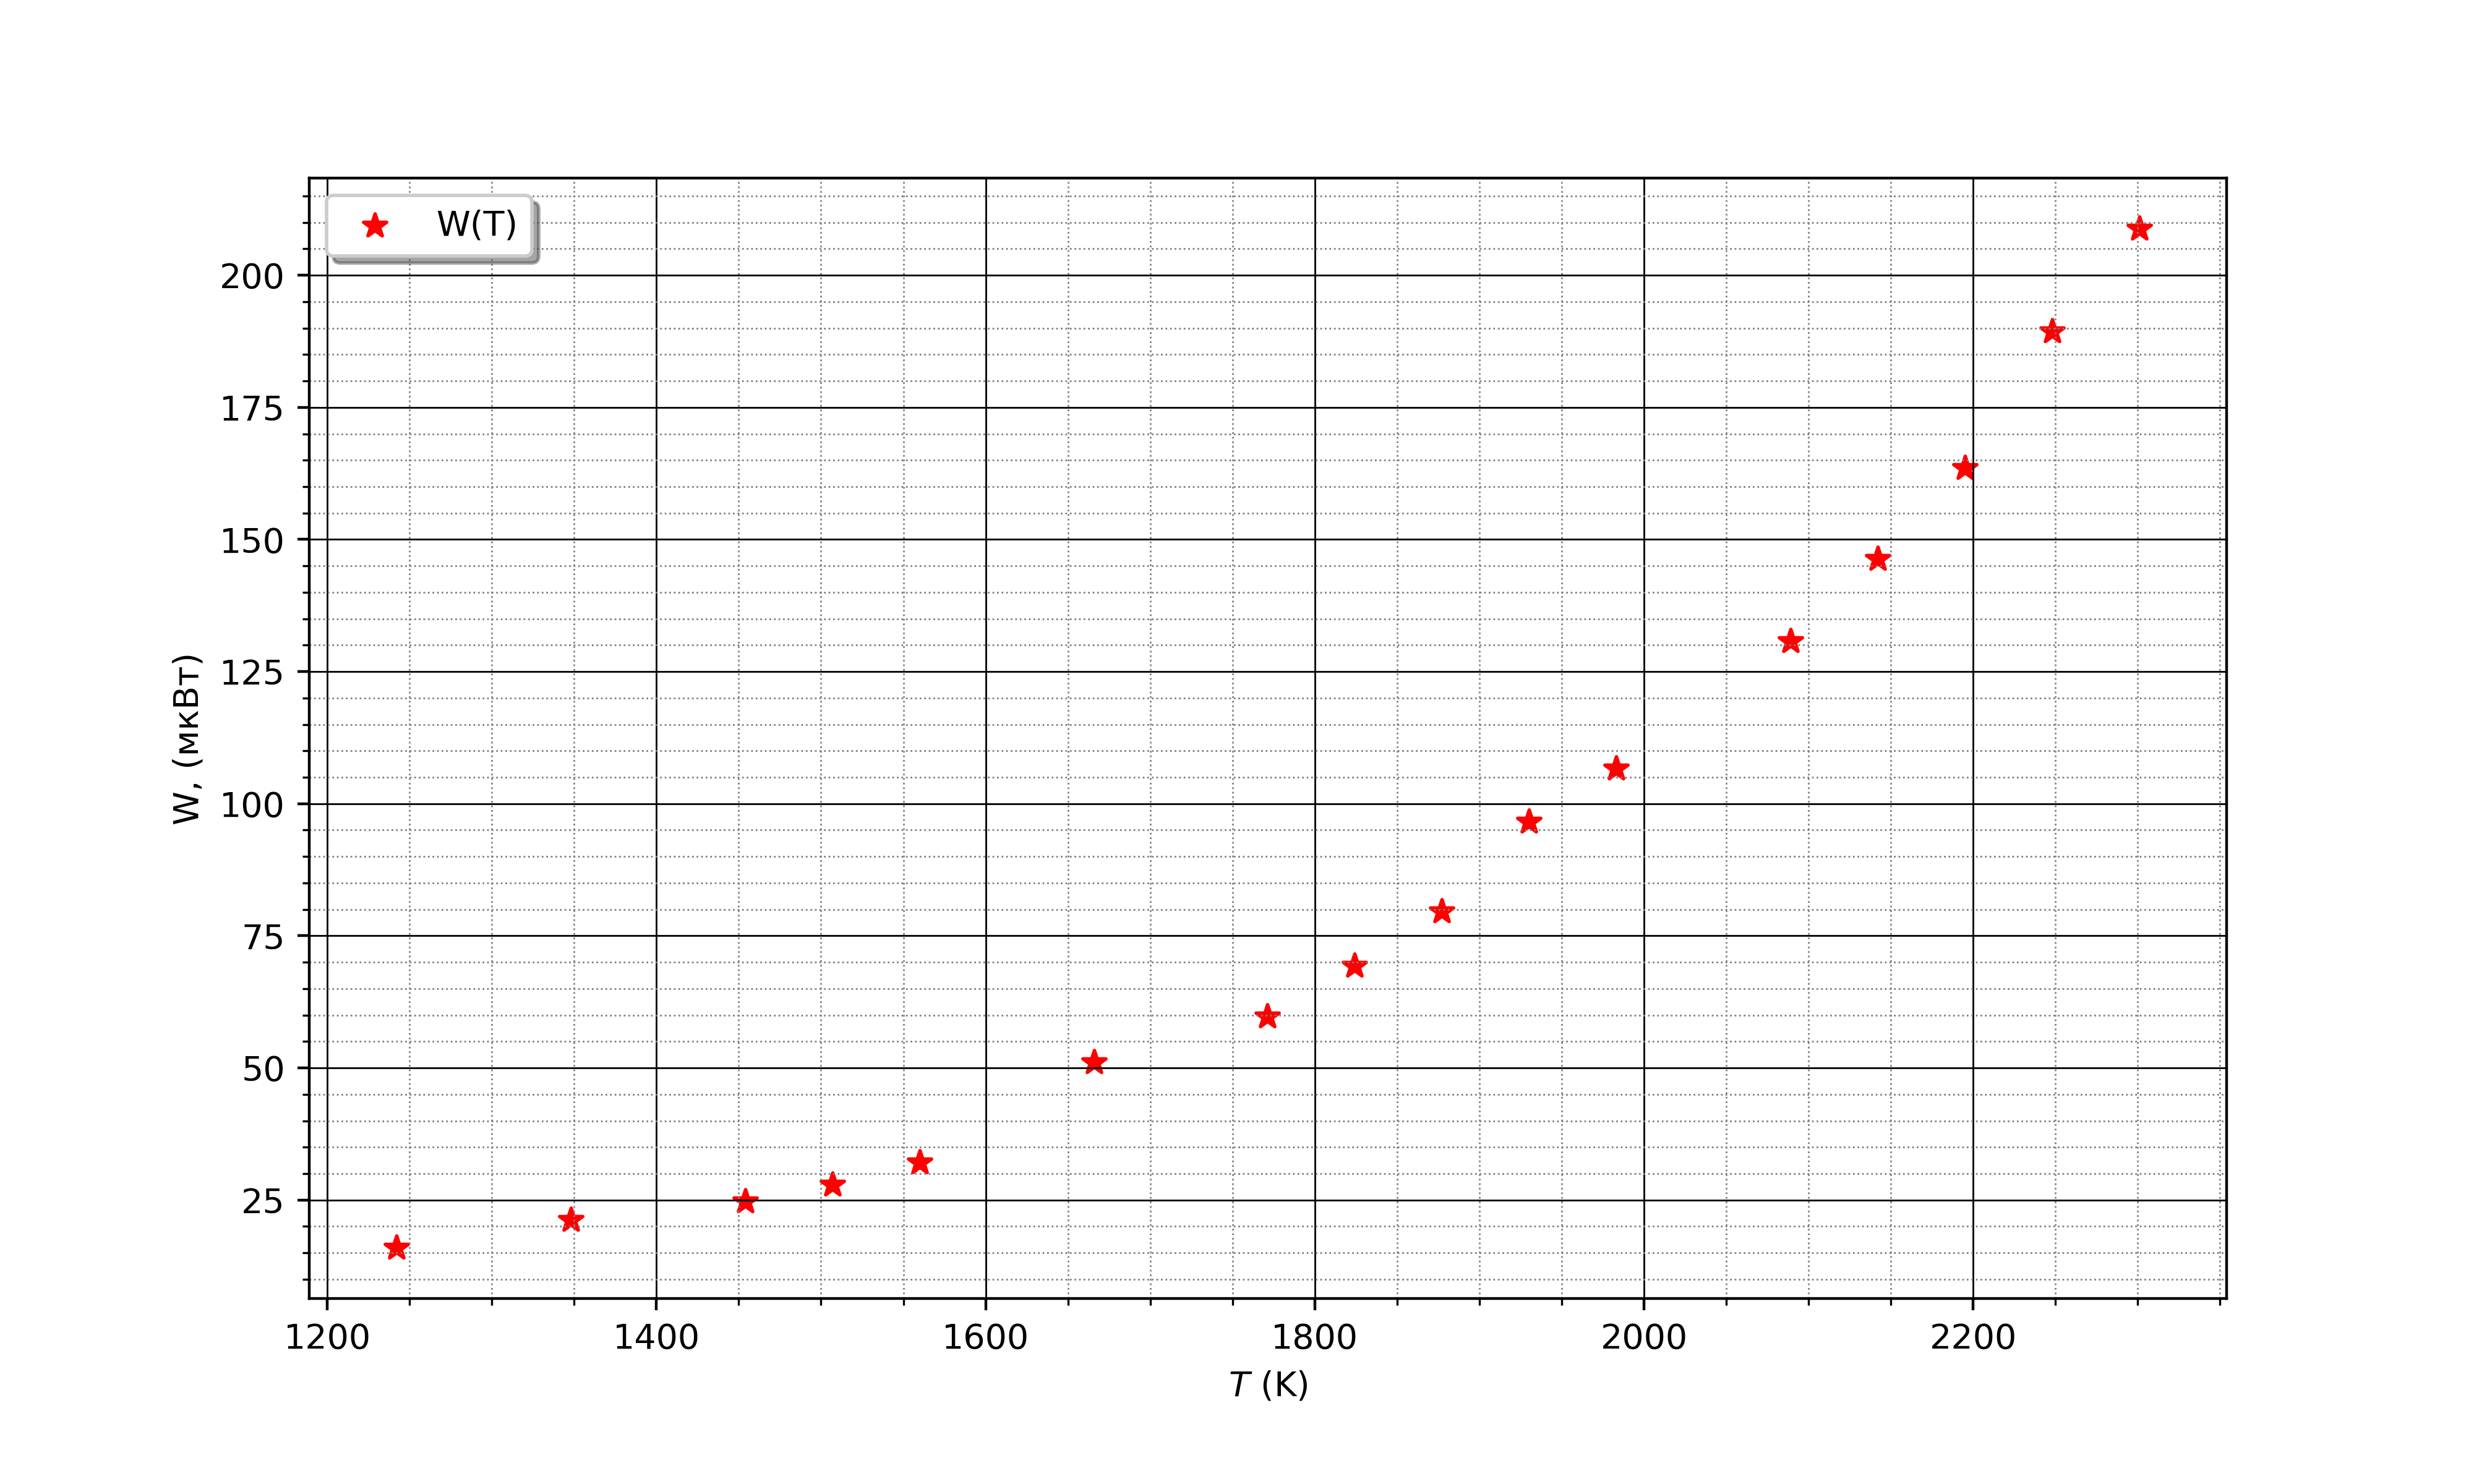
\includegraphics[scale = 0.5]{W(T).png}
        \caption{Зависимость мощности подаваемой на нить от ее термодинамической температуры}
        \label{graph1}
        \end{center}
    \end{figure}

    \item Преверим закон Стефана-Больцмана, построим в логарифмическом масштабе функцию $W = \varepsilon_T B T^n$,
    т.е. функцию
    $$\ln{W} = \ln{(\varepsilon_T B)} + n \ln{T}$$
    показана на рис. \ref{graph2}
    \begin{figure}[H]
        \begin{center}
        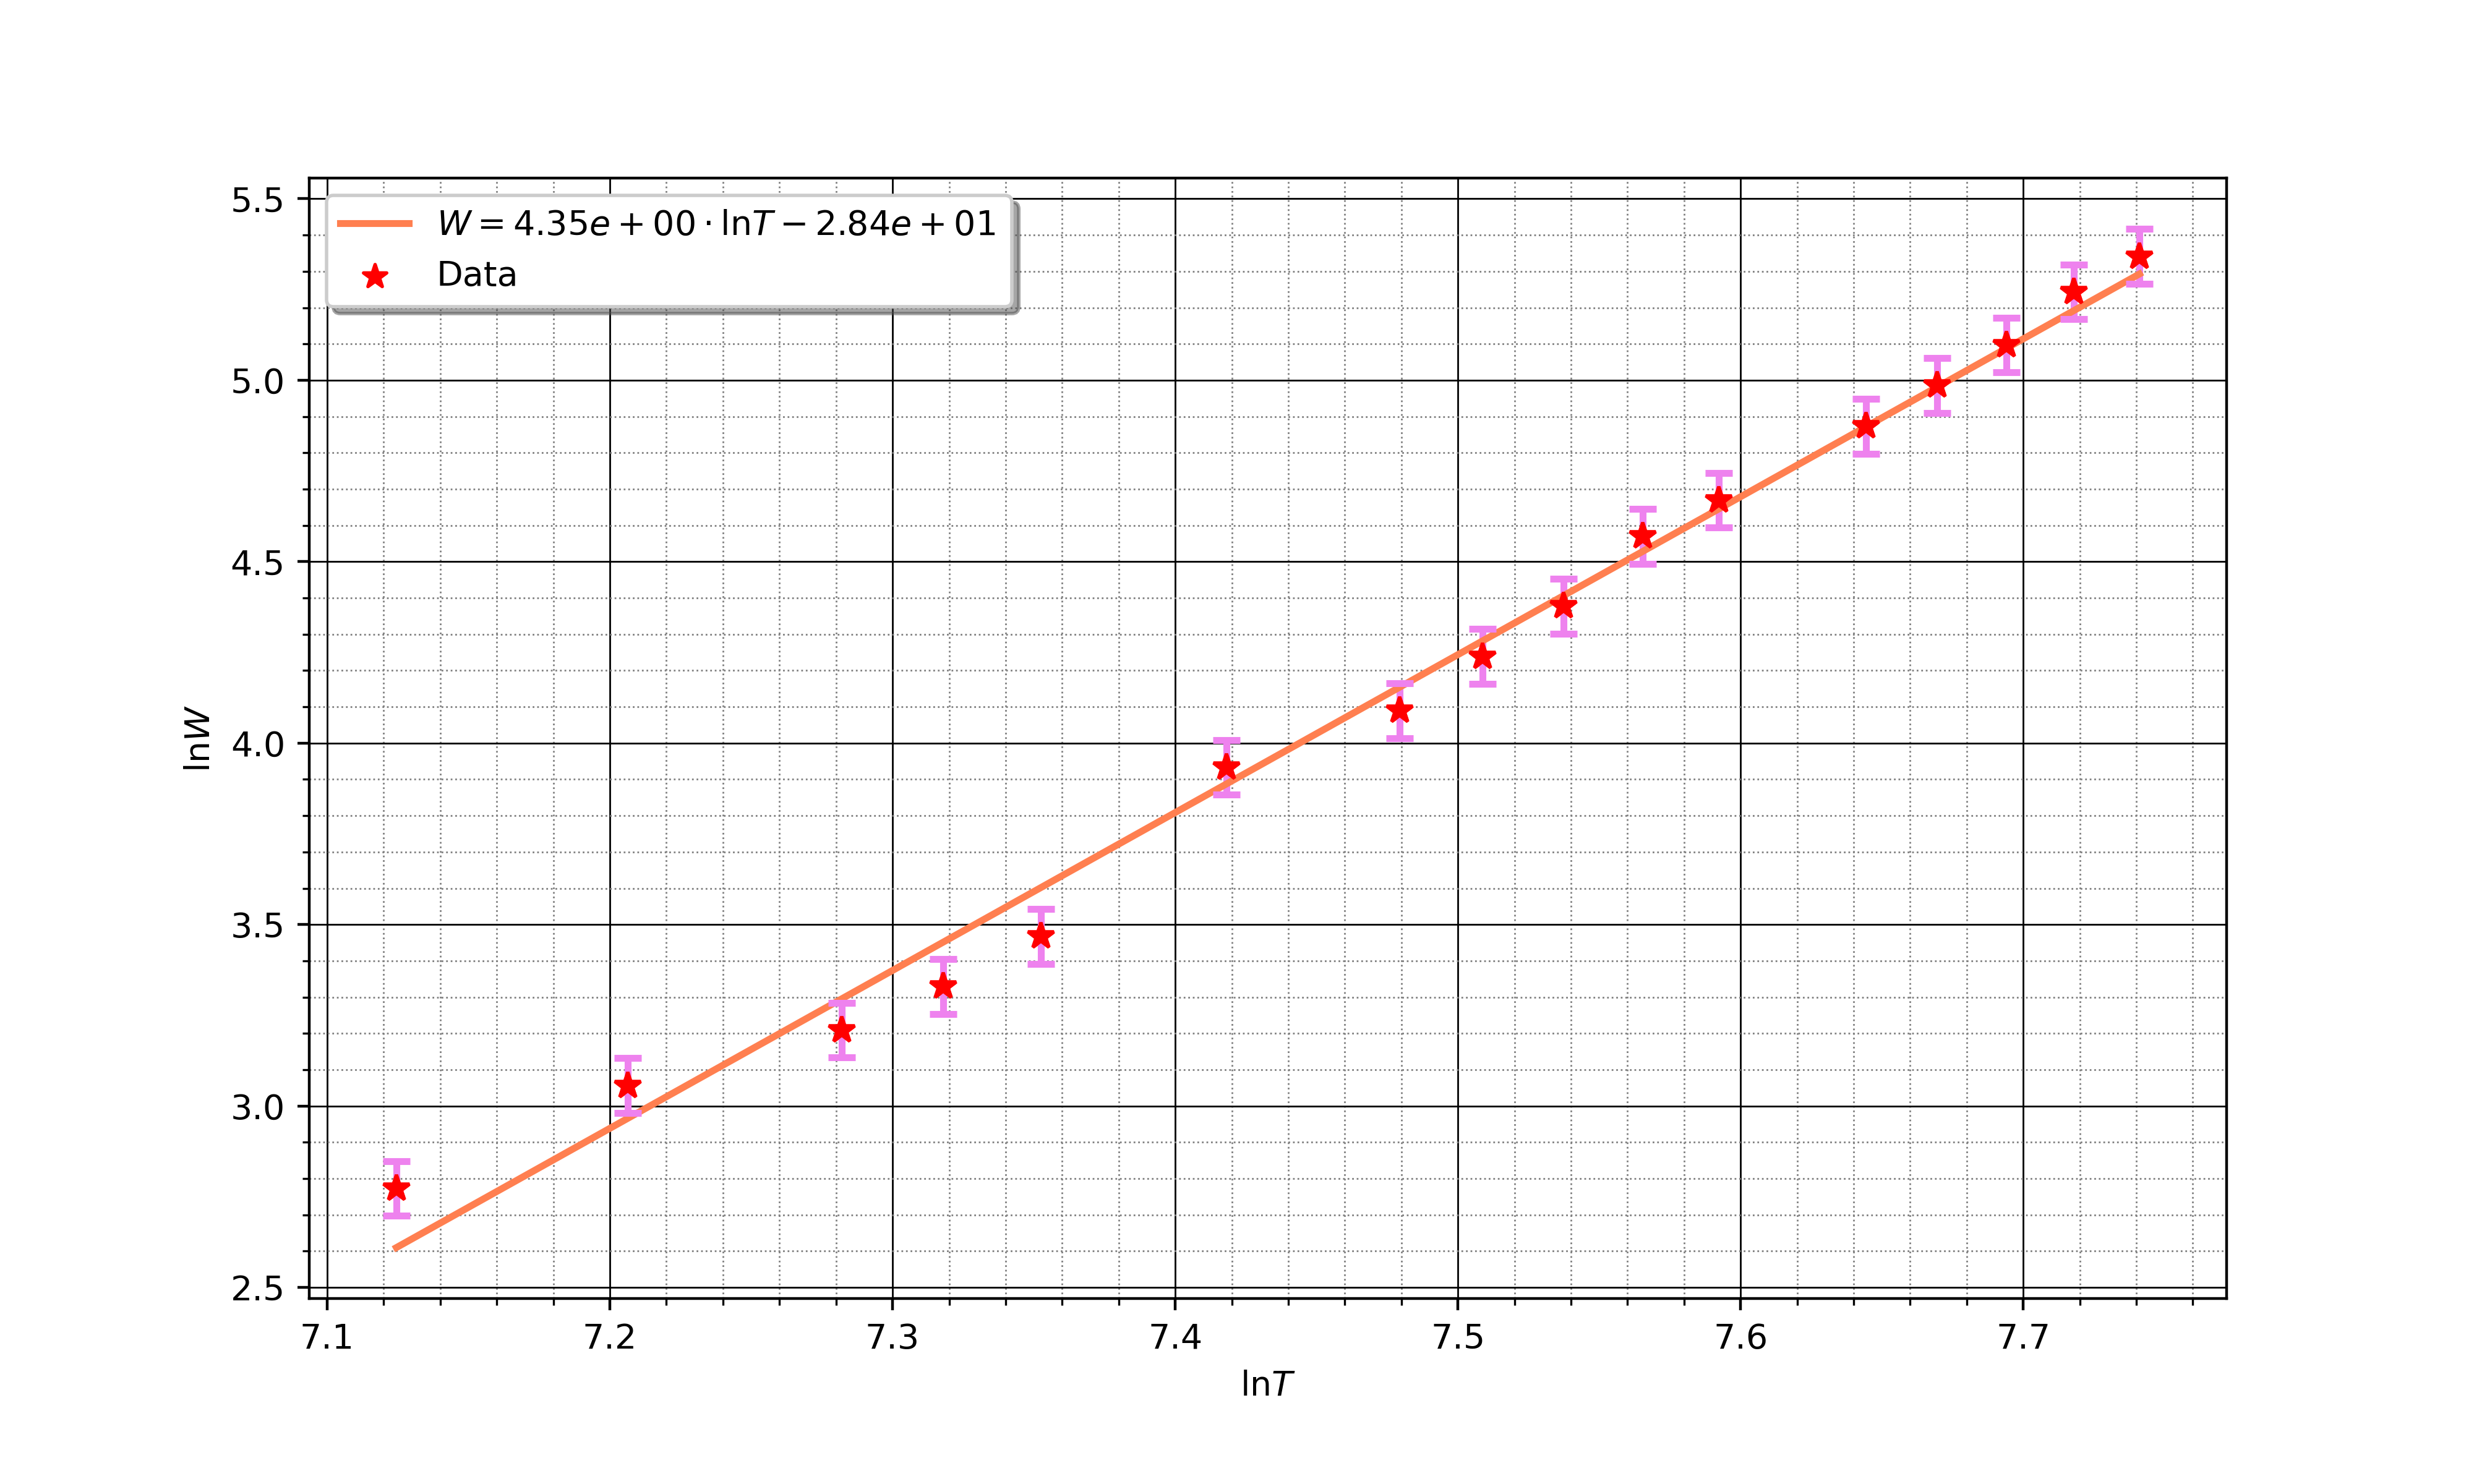
\includegraphics[scale = 0.5]{lnW.png}
        \caption{Зависимость мощности от температуры в логарифмическом масштабе}
        \label{graph2}
        \end{center}
    \end{figure}
    Откуда получаем значение $n = 4.35 \pm 0.11 (2.5 \%)$ \par 
    Сделаем фит этих данных с учетом, что показатель n = 4, покажем на рис. \ref{graph3}
    \begin{figure}[H]
        \begin{center}
        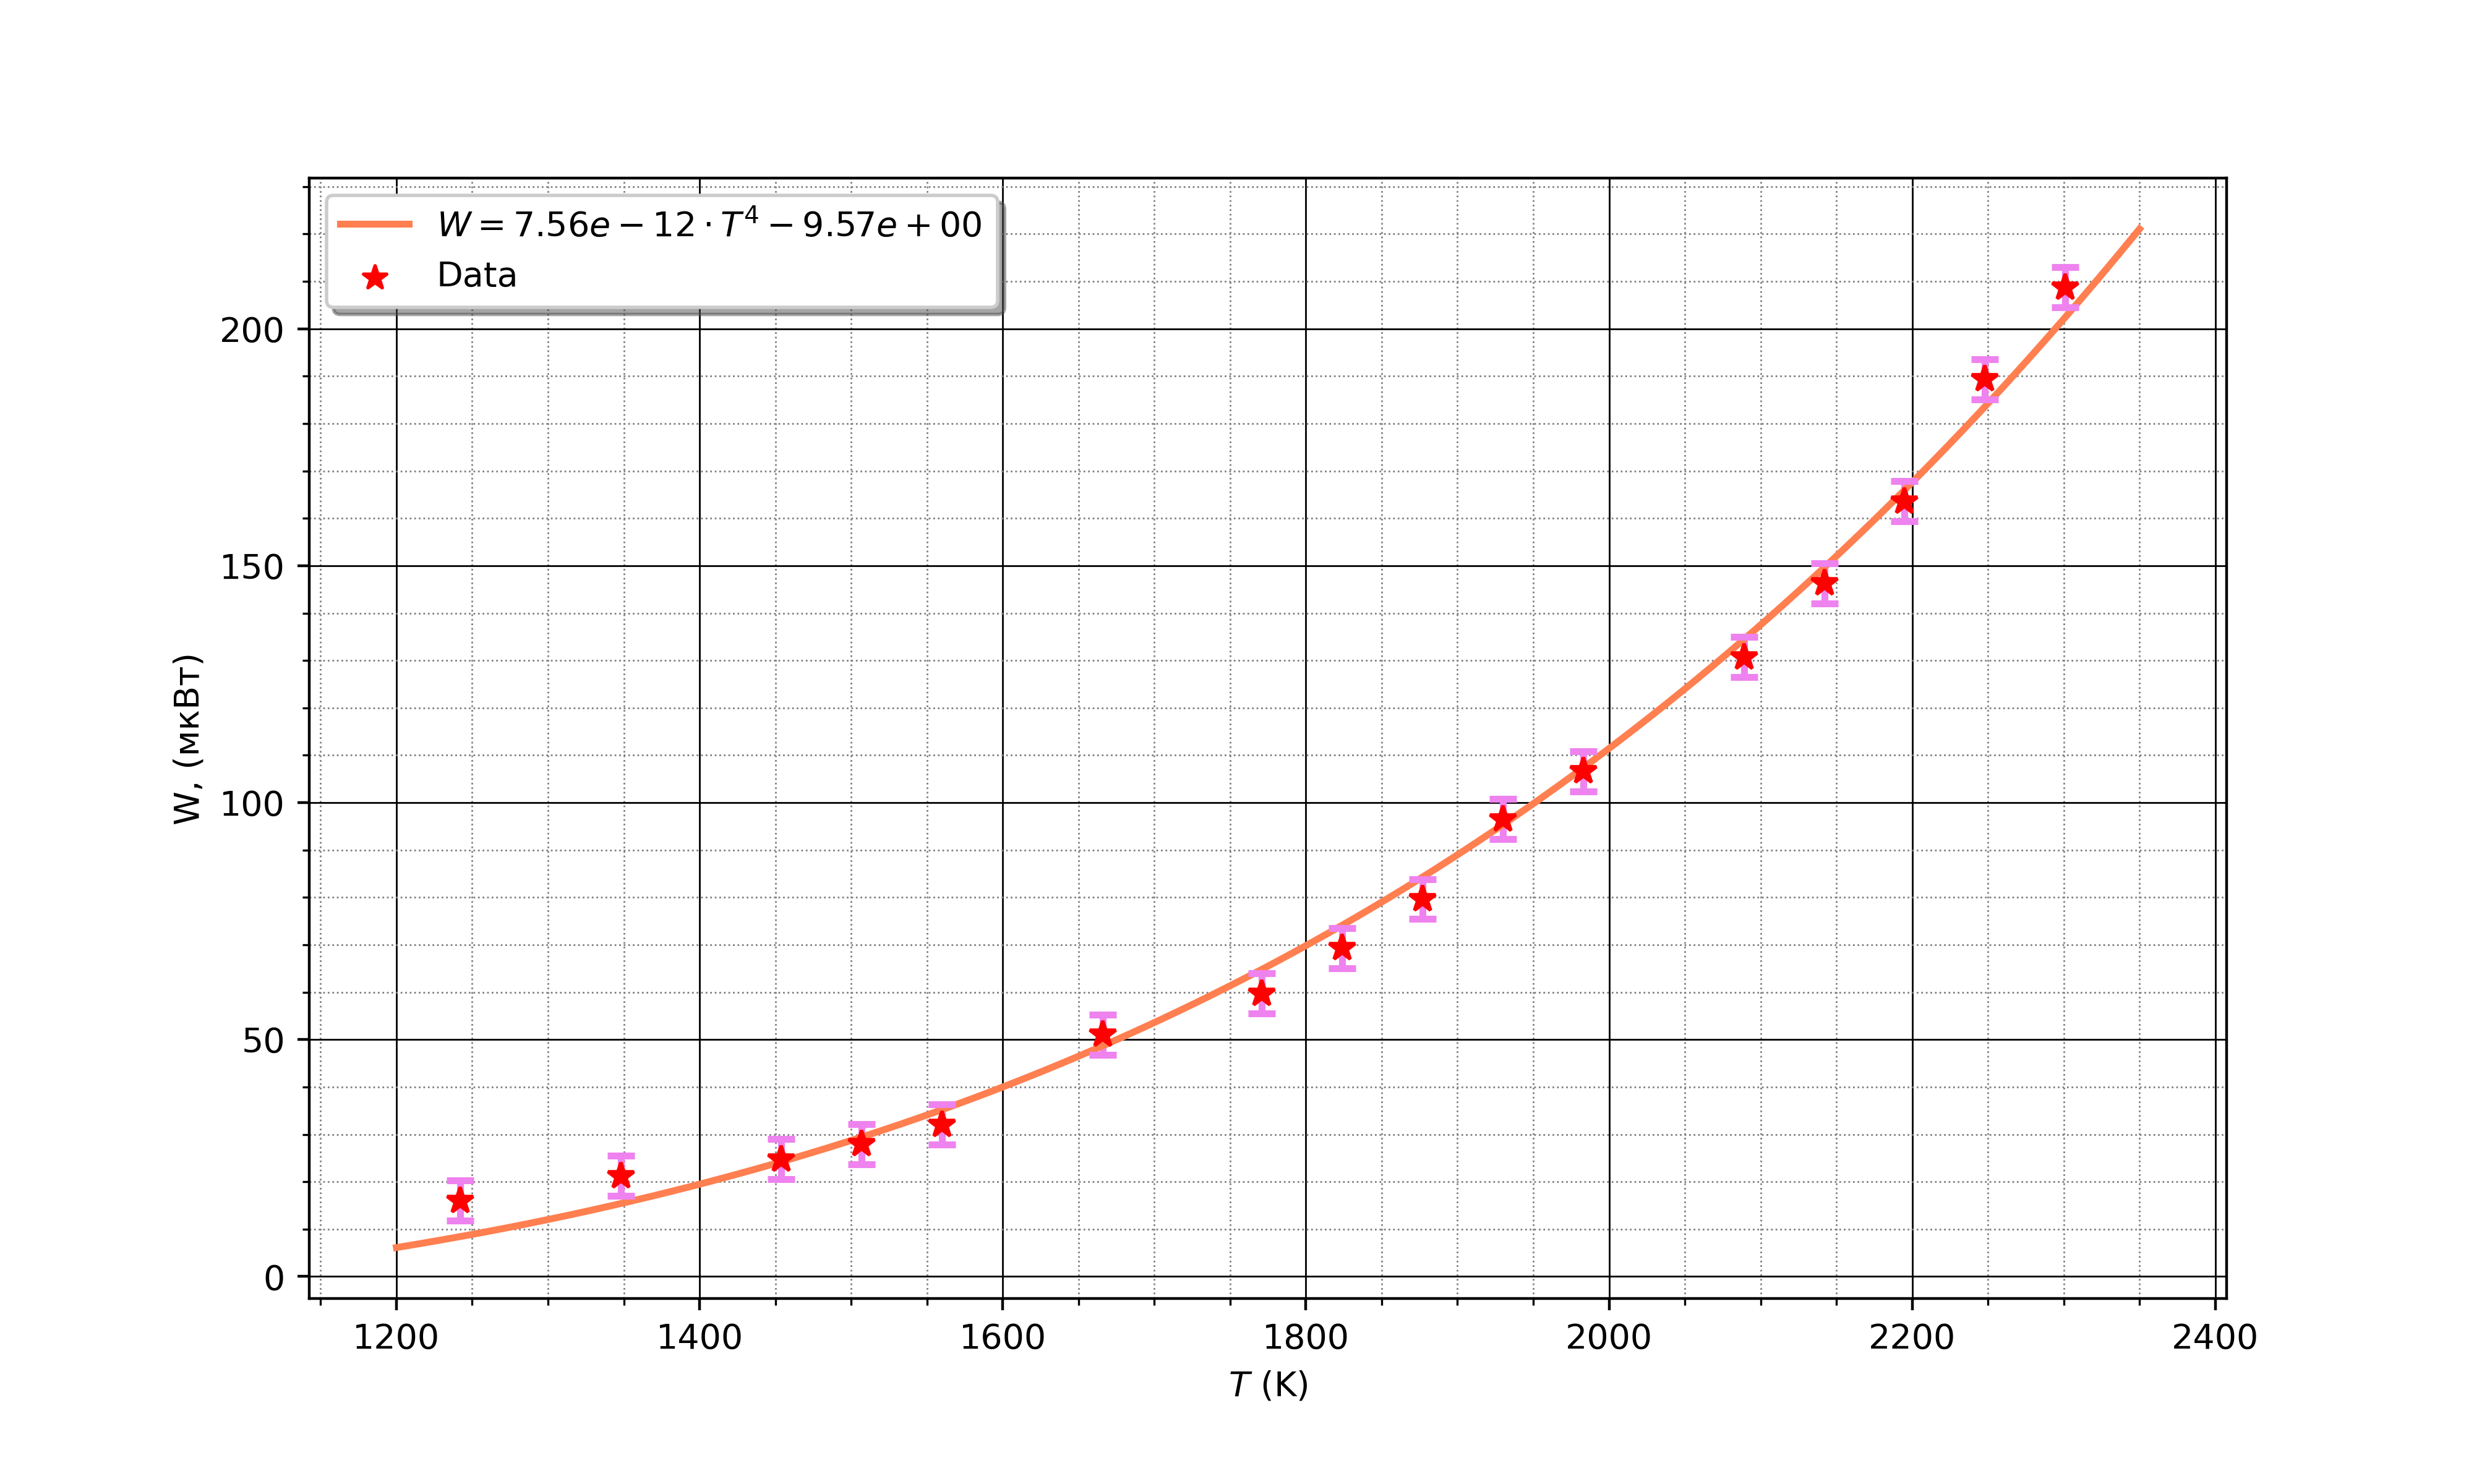
\includegraphics[scale = 0.5]{W(t)fit.png}
        \caption{Фит данных W(T)}
        \label{graph3}
        \end{center}
    \end{figure}
    Откуда $\varepsilon_T S \sigma \approx 7.56 \cdot 10^{-12} \; \left ( \frac{\text{Вт}}{m \cdot K^4} \right )$

    \item Найдем величину постоянной Стефана-Больцмана по формуле:
    $$\sigma = \frac{W}{\varepsilon_T S T^4}$$
    для каждого измеренного значения и усредним.
    $$\sigma = (101.98 \pm 1.44 )\cdot 10^{-11} \left ( \frac{\text{Вт}}{m \cdot K^4} \right ) \; (\pm 1.4\%)$$

    \item По формуле $h = \sqrt[3]{\frac{2 \pi^5 k_{\text{Б}^4}}{15 c^2 \sigma}}$ найдем постоянную Планка:
    $$h = (252.7 \pm 1.2) \cdot 10^{-35} (\text{Дж} \cdot c) \; (\pm 0.5 \%)$$

\end{enumerate}


\subsection{Измерение яркостной температуры неоновой лампочки}

Направим пирометр на неоновую лампочку и измерим пирометром яркостную температуру неоновой лампочки.
$$t \approx 960 \; ^{\circ}C$$

Однако если дотронемся пальцем до лампы, то обнаружим, что ее термодинамическая температура сильно ниже яркостной.
Дело в том, что неоновая лампа совсем не является моделью черного тела и ее излучение носит совсем другую природу - 
переход жлектронов между жнергетическими уровнями. Цвет - лишь совпадение.



\section{Вывод}

В ходе работы изучили модели АЧТ и серого тела. Ознакомились с принципами работы пирометра. Выяснилось, что термодинамическая
температура может не совсем не совпадать с яркостной. Проверили закон Стефана-Больцмана, на примере вольфрамовой нити вычислили
постоянные Планка и Стефана-Больцмана. В работе есть несовпадение теоретических констант с жкспериментальными ввиду измерений "на глаз"
при сравнении яркости нити накала в пирометре с яркостью обьектов исследования.















\end{document}